\chapter{Sequence Learning}
\label{chapter:sequence_learning}
In this chapter we delve into the models used when data is in the form of sequences of variable length. Sequential variable-length data require models that do not make assumptions on the length of the inputs. For example, standard dense linear layers cannot work on variable-length inputs, since the linear layer has a set number of input neurons.

In section~\ref{sec:recurrent_neural_networks} we discuss Recurrent Neural Networks (RNNs), which are sequential models that can be applied to variable-length input data. We cover the most common kind of RNN, the Long Short-Term Memory (LSTM) model, and briefly mention some alternatives.

In section~\ref{sec:sequence_alignments} we discuss how sequential protein data  within a single protein family can be manipulated to avoid the problem of variable-length data altogether, with some other disadvantages as a trade-off.

\todo{general stuff about next sequence element prediction}

% Finally, we discuss the transformer model?

\section{Recurrent Neural Networks}
\label{sec:recurrent_neural_networks}
In regular neural networks, we usually think of the input being given to the model, going through a layer which produces an output, which is then fed to the \textit{next} layer of the model. This continues until the data reaches the final layer, which produces the final output.

A recurrent neural network (RNN) is a layer that \textit{recurs} in the model -- for the purposes of RNNs, this refers to the input being processed by the RNN, producing an output, which is then fed into the RNN again, usually in combination with more data. For sequential data, this ``more data'' is usually the next element of the sequence. This enables processing of variable-length data, by making the RNN produce a ``hidden state'' as it processes the sequence. The RNN starts with an initial hidden state, typically initialized to a zero vector. It then takes this hidden state and the first element of the sequence and processes it in some way, to produce the next hidden state. It repeats this process with the new hidden state and the next element of the sequence, until there are no elements in the sequence left. The intermediate hidden states can be thought of as the RNN's ``memory'' about the sequence seen so far. The final hidden state can then be considered the output of the RNN, or one can use the sequence of the intermediate hidden states as an output, depending on the application.

More formally, consider a sequential datapoint $X = (x_1, x_2, \dots, x_n)$. An RNN can be seen as a function $\mathrm{RNN} \colon \prts{\mathbb{R}^h, \mathbb{R}^l} \to \mathbb{R}^h$, where $h$ is the size of the hidden state (a hyperparameter) and $l$ is the size of each $x_i$ of $X$. To apply the RNN on the entire sequence as described above would mean evaluating the following:
\[h_n = \mathrm{RNN}\prts{\mathrm{RNN}\prts{\dots \mathrm{RNN}\prts{\mathrm{RNN}\prts{h_0, x_1}, x_2} \dots, x_{n - 1}}, x_n}\]
Where $h_0$ is the initial hidden state (usually simply $\ve{0}$) and $h_n$ is the final hidden state of the RNN after processing the entire sequence. The $\operatorname{RNN}$ function can be defined in many, many ways, but a few popular options have become commonplace. This includes RNNs like the Long Short-Term Memory (LSTM) or the Gated Recurrent Unit (GRU).

Figure \ref{fig:rnn_comparison} shows a comparison of regular neural networks and RNNs. It also illustrates the concept of ``unrolling'' an RNN. The RNN as shown in figure \ref{subfig:rnn} is a recurrent model, that takes its own output as an input. However, if you unwind the recursion over the entirety of the input sequence, you reach figure \ref{subfig:rnn_unrolled}, which more accurately and explicitly shows how an RNN functions. Note that even though the RNN is drawn multiple times in the unrolled version, it is the same model used again and again.

\begin{figure}[ht]
    \centering
    \begin{subfigure}[t]{0.48\linewidth}
        \centering
        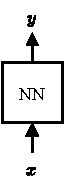
\includegraphics[scale = 1.35]{report/figures/nn.pdf}
        \caption{Regular neural network.}
        \label{subfig:nn}
    \end{subfigure}%
    \hfill
    \begin{subfigure}[t]{0.48\linewidth}
        \centering
        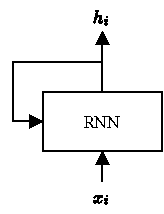
\includegraphics[scale = 1.35]{report/figures/rnn.pdf}
        \caption{Recurrent neural network.}
        \label{subfig:rnn}
    \end{subfigure}
    
    \begin{subfigure}[t]{1\linewidth}
        \centering
        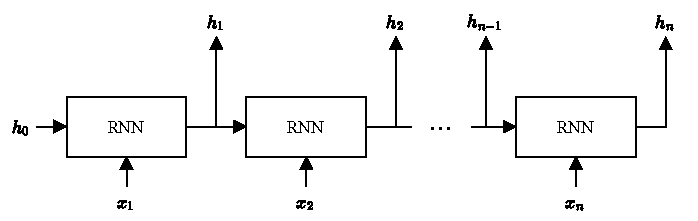
\includegraphics[scale = 1.35]{report/figures/rnn_unrolled.pdf}
        \caption{Unrolled recurrent neural network.}
        \label{subfig:rnn_unrolled}
    \end{subfigure}
    \caption{\subref{subfig:nn}~A regular neural network usually takes a single input and produces a single output. \subref{subfig:rnn}~A recurrent neural network takes a sequence as input, processing each element one at a time, feeding the intermediate hidden states as input to the next recursive call of the RNN. The RNN's output can be considered the last hidden state $\prts{h_n}$ or the entire sequence of hidden states. \subref{subfig:rnn_unrolled}~An ``unrolled'' RNN, more explicitly showing the sequential inputs and the intermediate hidden states.}
    \label{fig:rnn_comparison}
\end{figure}

\subsection{Long Short-Term Memory}
The Long Short-Term Memory (LSTM) is a recurrent neural network (RNN) which uses several \textit{gates} to control how to manipulate the input hidden state based on the input sequence element.

In contrast to some other RNNs, the LSTM actually utilizes two inner states of the same size, where one is known as the ``cell'' state and another is the hidden state. Thus the LSTM can be explained as the function $\mathrm{LSTM} \colon \prts{\prts{\mathbb{R}^h, \mathbb{R}^h}, \mathbb{R}^l} \to \prts{\mathbb{R}^h, \mathbb{R}^h}$ which has the definition \cite{pytorchnn}
\begin{align*}
    \mathrm{LSTM}\prts{\prts{c_{i - 1}, h_{i - 1}}, x_i} &= \prts{c_i, h_i} \\
    c_i &= F_i * c_{i - 1} + I_i * G_t \\
    h_i &= O_i * \tanh\prts{c_i} \\
    F_i &= \mathrm{\sigma}\prts{\mathrm{L_1}\prts{x_i} + \mathrm{L_2}\prts{h_{i - 1}}} \\
    I_i &= \mathrm{\sigma}\prts{\mathrm{L_3}\prts{x_i} + \mathrm{L_4}\prts{h_{i - 1}}} \\
    G_i &= \tanh\prts{\mathrm{L_5}\prts{x_i} + \mathrm{L_6}\prts{h_{i - 1}}} \\
    O_i &= \mathrm{\sigma}\prts{\mathrm{L_7}\prts{x_i} + \mathrm{L_8}\prts{h_{i - 1}}}
\end{align*}
where $O_i$, $G_i$, $F_i$ and $I_i$ are the ``gates'', known as the output gate, cell gate, forget gate and input gate respectively. $\operatorname{\sigma}$ is the sigmoid function while $*$ denotes element-wise multiplication. Each $\mathrm{L_i}$ denotes a linear transformation of the form
\[\mathrm{L_i}\prts{x} = W_i x + b_i\]
where $W_i$ and $b_i$ are learnable parameters of the model, denoted as weight and bias respectively -- thus each $\mathrm{L_i}$ denotes what is otherwise known as a dense linear layer with bias.

The above formal definition is perhaps not the most instructive. Figure \ref{fig:lstm_structure} shows a diagram of the structure of the LSTM. Intuitively, the gates can be understood as operations on the internal ``memory'' of the LSTM (its states). The forget gate $F_i$ can be thought of as deciding what to remove or ``forget'' from the cell state. The input gate $I_i$ and the cell gate $G_i$ then decide what to add to the ``memory'' of the cell state. Finally, the output gate $O_i$ decides how to combine the resulting new cell state $c_i$ and the previous hidden state $h_{i - 1}$ into a new hidden state $h_i$.

\begin{figure}[ht]
    \centering
    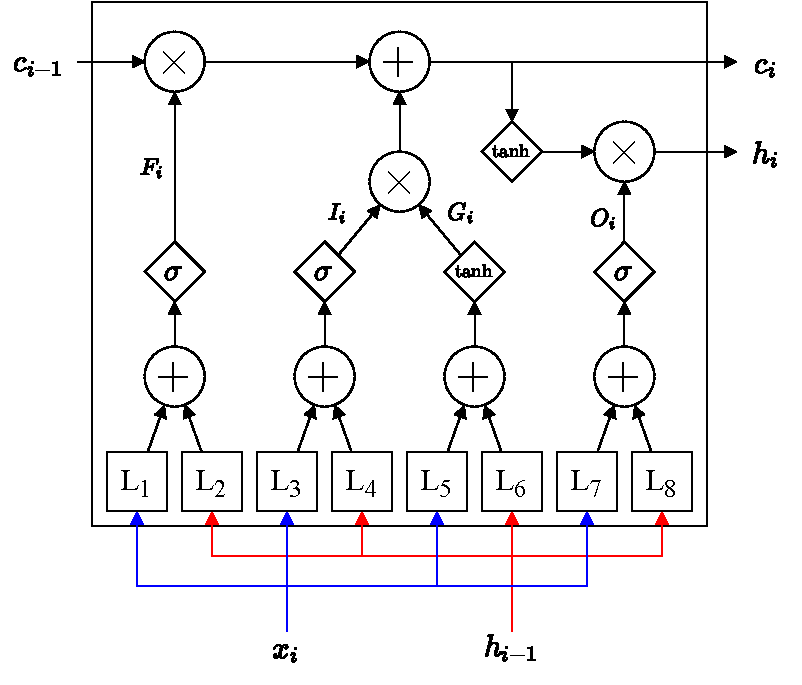
\includegraphics{report/figures/lstm.pdf}
    \caption{The structure of the LSTM, taking $c_{i - 1}$, $h_{i - 1}$ and $x_i$ as inputs, and returning $c_i$ and $h_i$. Squares indicate dense linear layers, diamonds indicate element-wise non-linear activation functions and circles denote binary element-wise operators. Connections from $x_i$ and $h_{i - 1}$ coloured for clarity.}
    \label{fig:lstm_structure}
\end{figure}

The LSTM was designed to avoid the common problem of vanishing gradients in neural networks. This problem is especially prevalent in RNNs, because the repeated application of the RNN leads to a very deep computational graph, in which gradients have to be backpropogated. Due to the depth of this graph, the gradient has a tendency to either vanish or explode. Note how the LSTM actually does not perform a lot of operations on the cell state $c_{i - 1}$. This helps prevent the vanishing gradient problem.

\subsection{Other Recurrent Neural Networks}
There are many other types of RNNs. One of the earliest RNNs was proposed by Jeffrey Elman \cite{elman1990finding}, and consists simply of the following computation \cite{pytorchnn}:
\[\mathrm{Elman}\prts{h_{i - 1}, x_i} = h_i = \tanh\prts{\mathrm{L_1}\prts{h_{i - 1}} + \mathrm{L_2}\prts{x_i}}\]
Where each $\mathrm{L_i}$ again denotes a linear layer, as above.

Another common RNN is the Gated Recurrent Unit (GRU) which, like the LSTM, uses gates to regulate the internal state of the RNN. The GRU however has a somewhat simpler architecture and uses only a single state. The simpler architecture makes the GRU less computationally expensive, and further helps to prevent vanishing or exploding gradients, in comparison to the LSTM. The GRU consists of the following computations \cite{pytorchnn}:
\begin{align*}
    \mathrm{GRU}\prts{h_{i - 1}, x_i} &= h_i \\
    h_i &= z_i * h_{i - 1} + \prts{1 - z_i} * n_i  \\
    z_i &= \mathrm{\sigma}\prts{\mathrm{L_1}\prts{x_i} + \mathrm{L_2}\prts{h_{i - 1}}} \\
    n_i &= \tanh\prts{\mathrm{L_3}\prts{x_i} + r_i * \mathrm{L_4}\prts{h_{i - 1}}} \\
    r_i &= \mathrm{\sigma}\prts{\mathrm{L_5}\prts{x_i} + \mathrm{L_6}\prts{h_{i - 1}}}
\end{align*}
In the above, $r_i$, $z_i$ and $n_i$ are referred to as the \textit{reset}, \textit{update} and \textit{new} gates, respectively. Intuitively, the gates can be thought of a method for the GRU to cleverly interpolate between a newly constructed hidden state $\prts{n_i}$ and the old hidden state. It makes this interpolation using the update gate's result, $z_i$. The reset gate roughly decides what to keep/forget from the old hidden state when constructing the new one.

There are many more RNNs, of which many are variations of the above. For example, the multiplicative LSTM (mLSTM) \cite{krause2016multiplicative} extracts certain information from the previous hidden state, which it then uses in the LSTMs gates, instead of the previous hidden state. That is, it calculates
\[m_i = \mathrm{L_{m_1}}\prts{x_i} * \mathrm{L_{m_2}}\prts{h_{i - 1}}\]
and then uses $m_i$ instead of $h_{i - 1}$ in the gates of the LSTM.

\section{Sequence-to-Sequence Models versus Bottleneck Models}
\label{sec:seq2seqvsbottleneck}
As mentioned above, an RNN's output may be considered either its last hidden state $h_n$, or the entire sequence of resulting hidden states $\prts{h_1, \dots, h_n}$.

In the case of the last hidden state, the model produces a ``bottleneck''; It forces the sequence through a representation of a fixed size, which is small in the sense that it does not depend on the length of the input sequence. For such a model, a compact representation is readily available in the form of the bottleneck layer. We say that the model up to the bottleneck layer encodes the sequence to the bottleneck and is as such known as the encoder. In order to facilitate conversion from the bottleneck representation back to a sequence (which is useful if you want to explore the space of representations) and in order to ensure that the representation holds the most essential features of the sequence, a model (the decoder) is trained to decode the representation back to the input sequence -- thus we reach the concept of an auto-encoder. The decoding of a representation into a variable-length sequence is however very difficult for a model to learn and perform correctly to an acceptable degree. In section \ref{sec:sequence_alignments} we will see how this problem may be circumvented.

In the case of the entire sequence of hidden states as the output, we say that the RNN is a ``sequence-to-sequence'' model, since it takes one sequence of some length $n$ and produces another sequence of the same length\footnote{It is possible to have sequence-to-sequence models which produce sequences of another length than the input, but this is more relevant to natural language processing and not as relevant to protein processing.}. A compact, fixed-size representation is not as easily obtained from the resulting sequence as in the case of bottleneck models, since there is no obvious canonical way to reduce the sequence to such a representation. The sequence could be reduced in many different ways, but this is not always desired, as the translation back to a sequence becomes more complicated or impractical, depending on the way the reduction is done.

It's not obvious which of the above two approaches should be preferred. Bottleneck models easily provide a compact representation, but such a representation is hard to decode back to a variable-length sequence. Sequence-to-sequence models don't need a decoder, since they produce a sequence out of the box -- however, obtaining a compact representation is more difficult. We will explore both bottleneck models, in the form of the variational autoencoder, and sequence-to-sequence models in the form of models based on RNNs or other methods.

RNNs are just one type of sequence-to-sequence models. There are other types of models that can be used to process sequences into new sequences. For example, convolutional neural networks (CNNs) can also do this. CNNs are known for their ability to process images, but sequences work just as well -- one could after all just consider a sequence as a 1-dimensional image. Making a sequence-to-sequence model based on CNNs simply involves appropriately padding the input, so that the resulting output remains the same length as the original sequence. Then it is only a question of how exactly the convolution is applied to the sequence. We will explore one such method in section \ref{sec:wavenet_model}.

% EMIL: uncommented
% Another possibility is attention-based models. Attention is a general mechanism which can be applied to sequence-to-sequence models, but it is most famously utilized in the Transformer model \cite{vaswani2017attention}. The Transformer uses a mix of linear layers and so-called ``self-attention'' layers to encode and decode the input sequence. Despite the presence of an encoder and decoder, the Transformer never reduces the sequence into a fixed-length representation, so it is not a bottleneck model. We will explore the Transformer in more detail in section \ref{sec:transformer_model}.

\section{Sequence Alignments}
\label{sec:sequence_alignments}
As proteins are sequential in nature, RNNs can be used to integrate them into deep learning models. However, despite RNNs being suited for sequential data, it is not always the best model to use for proteins. While RNNs are able to process proteins, there are certain disadvantages in the way that RNNs do processing. For example, when an RNN processes a single amino acid, it cannot take into account any remaining amino acids of the protein, because it has not reached those amino acids yet, even though it may be worthwhile to consider both previous and future amino acids. Also, the RNN cannot directly take into account the sequence seen so far -- it can only use the hidden state up to a certain point, which is only a compact representation of the sequence so far.

A model which could directly take into account the entire rest of the sequence when making a prediction could potentially perform better. It would be difficult to make such a model work with variable-length data however. Fortunately, it is possible to convert a family of proteins into a fixed-length number of sequences, by performing a \textit{sequence alignment}.

Recall the introduction on protein families in section \ref{sec:protein_families}. Through evolution, proteins become related in families. Consider training a model on a single protein family. Because the proteins are related, they have certain similarities. As it turns out, we may use these similarities to our advantage when training our model. A sequence alignment attempts to align the parts of the proteins in a family which appear similar, while placing gaps to accommodate for the required ``stretching'' of the proteins.

As a toy example, consider the top part of figure \ref{fig:sequence_alignment_toy_example}. The original sequence \texttt{ABCDEFGH} evolves to 3 other sequences, where one has the \texttt{B} changed to an \texttt{L}, another has the \texttt{E} removed and the last has a \texttt{K} inserted between the \texttt{F} and \texttt{G}. These changes are supposed to represent random mutations. One of the sequences then evolves further, resulting in a total of 6 different sequences.

An example of a sequence alignment of this toy protein family can be seen in the bottom part of figure \ref{fig:sequence_alignment_toy_example}. As can be seen, the sequence alignment attempts to line up the parts of the sequences that match the evolutionary history -- that is, the insertion and removal of amino acids causes gaps to be inserted into the other sequences, to keep the similar parts of the proteins at the same position.

\begin{figure}[ht]
    \centering
    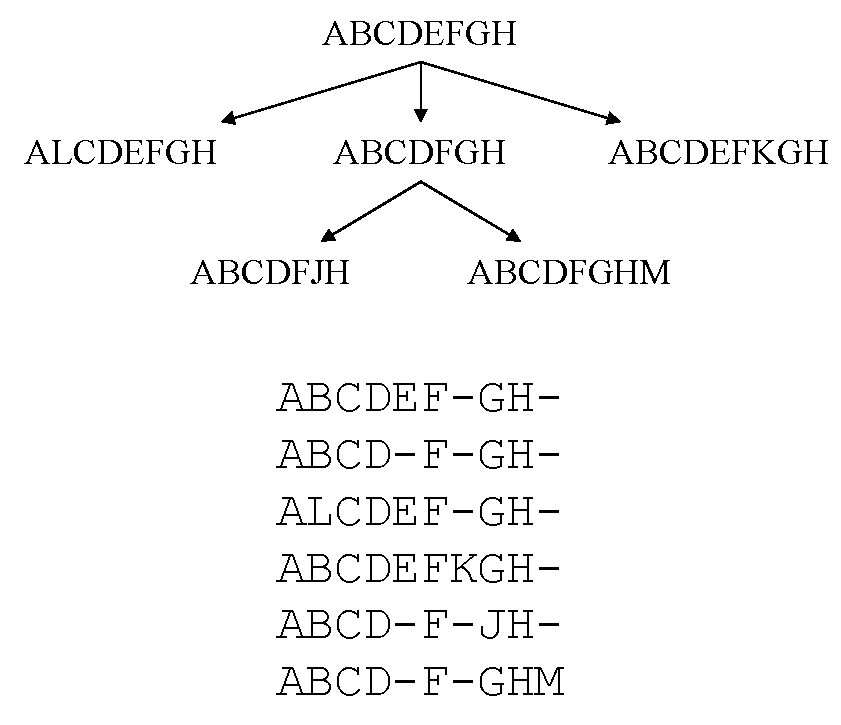
\includegraphics{report/figures/sequence_alignments.pdf}
    \caption{A toy example of a tiny protein family's evolution and an example sequence alignment. \todo{change to actual protein}}
    \label{fig:sequence_alignment_toy_example}
\end{figure}

Notice that the resulting sequence alignment causes all the sequences to be of the same length. Essentially, the sequence alignment provides absolute positions within the proteins, a luxury we did not have before. This is highly desirable, since it makes the choice of model much more flexible. We can now include models that only work on fixed-length data in our considerations.

For example, we can now apply densely connected linear layers to the sequences, since we now know the length of our data beforehand. This will prove to be very useful when we implement variational autoencoders in section \ref{sec:variational_autoencoders_experiement}.

However, sequence alignments are not perfect. There are significant disadvantages to using sequence alignments. First of all, the production of a sequence alignments requires the definition of a sort of scoring function, which basically optimizes the alignment based on how much an insertion of a gap or substitution costs. How exactly to decide on the specifics of the scoring function is not clear, making each alignment produced slightly different based on the parameters chosen. The toy example in figure \ref{fig:sequence_alignment_toy_example} is simple and the resulting alignment is obvious, but given thousands of sequences, the problem becomes much more complicated. Also, you may not have the evolutionary tree which resulted in the protein family (like we do in the toy example), which makes the analysis of the proteins much more complicated. As if it wasn't enough, multiple sequence alignment is also NP-hard \cite{wang1994complexity}, which means that an alignment must rely on heuristics and sub-optimal solutions in order to be tractable.

To actually produce an alignment, many parameters must be decided upon. There are many different methods and heuristics to choose from and the resulting alignment could be different depending on these choices. This makes the training of models on alignments difficult -- some alignments may be well-suited for training, while others may not, and it is difficult to tell the two apart.

Another problem with alignments is the way that they modify the underlying data. Fundamentally, protein data is variable-length. Changing this assumption involves the insertion of gaps. These gaps may change the proteins in ways that make it difficult for models to learn patterns that would otherwise have been easy if the gaps were not inserted.

Even worse, some alignments do not just insert gaps, they also cut away parts of the protein, or only preserve a certain section of the sequences. This is a much more destructive operation to the data, which may simply remove necessary sequence information.

Ideally, we wouldn't have to use sequence alignments, but sometimes an alignment leads to better training data than unaligned sequences. It also allows some additional choices for model architecture. The ``holy grail'' of protein modeling would be a model which does not require an alignment and can thus process variable-length sequences, while still being able to figure out the underlying protein structure and get some sense of absolute positions of the amino acids. Whether or not such a model is possible is very much an open question, which we will explore further in chapter \ref{chapter:experiments}. \todo{we actually do explore this right?}

%\todo{this is a conclusion, throw it away, save for later. Formulate as question instead and refer to chapter 6}

%Unfortunately, as we will see in chapter \ref{chapter:experiments}, we are still quite far from such a model.
